\hypertarget{_subject_to_8cpp}{}\section{/home/zheng/catkin\+\_\+ws/src/qp\+O\+A\+S\+E\+S-\/3.2.1/src/\+Subject\+To.cpp File Reference}
\label{_subject_to_8cpp}\index{/home/zheng/catkin\+\_\+ws/src/qp\+O\+A\+S\+E\+S-\/3.\+2.\+1/src/\+Subject\+To.\+cpp@{/home/zheng/catkin\+\_\+ws/src/qp\+O\+A\+S\+E\+S-\/3.\+2.\+1/src/\+Subject\+To.\+cpp}}
{\ttfamily \#include $<$qp\+O\+A\+S\+E\+S/\+Subject\+To.\+hpp$>$}\newline
Include dependency graph for Subject\+To.\+cpp\+:
\nopagebreak
\begin{figure}[H]
\begin{center}
\leavevmode
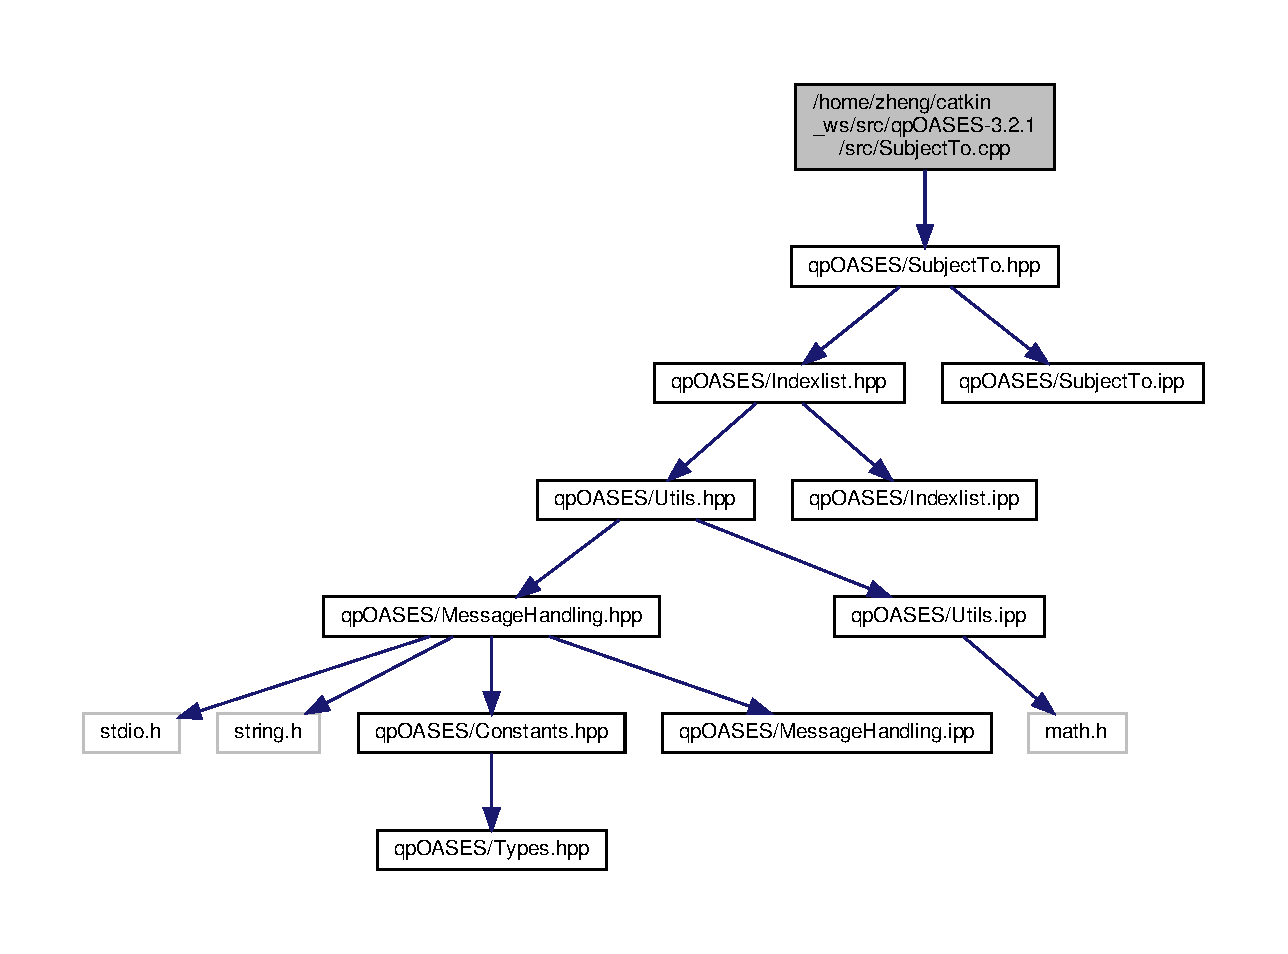
\includegraphics[width=350pt]{_subject_to_8cpp__incl}
\end{center}
\end{figure}


\subsection{Detailed Description}
\begin{DoxyAuthor}{Author}
Hans Joachim Ferreau, Andreas Potschka, Christian Kirches 
\end{DoxyAuthor}
\begin{DoxyVersion}{Version}
3.\+2 
\end{DoxyVersion}
\begin{DoxyDate}{Date}
2007-\/2017
\end{DoxyDate}
Implementation of the \hyperlink{class_subject_to}{Subject\+To} class designed to manage working sets of constraints and bounds within a \hyperlink{class_q_problem}{Q\+Problem}. 